\newpage

\section{Additional Analysis of Reference-Hint Selection}
\label{app:hint-selection}

This appendix expands on the two refinements introduced in
Section~\ref{sec:method-ectr}: $K$-marginalization of negative hints
(Appendix~\ref{app:negative-hint}) and excluding the target rollout from the
hint pool (Appendix~\ref{app:self-hint}). Together they detail why the vanilla
contrastive signal is unreliable and how each refinement restores a clean,
verifier-aligned signal.

\subsection{Negative-Hint Selection: Case Analysis and \texorpdfstring{$K$}{K}-Marginalization}
\label{app:negative-hint}

\paragraph{Why a single negative hint is unreliable.}
Correct solutions tend to converge to a small set of canonical strategies,
whereas incorrect solutions diverge across many distinct error modes. Whether
the optimization direction induced by the vanilla contrastive signal aligns
with the verifier therefore depends on whether the target rollout $y$ and the
sampled negative hint $y_w^*$ share a comparable error type.
Table~\ref{tab:naive-failure-cases} enumerates the three resulting cases:
\begin{itemize}
    \item \textbf{Correct $y$.} The teacher endorses each token in $y$ under $y_c^*$ (driving $e_{c,t}$ up) and conflicts under $y_w^*$ (driving $e_{w,t}$ down), giving a strongly positive $e_{\text{ctr},t}$ that matches the verifier.
    \item \textbf{Incorrect $y$ with similar-error $y_w^*$.} Symmetrically, $e_{c,t}$ drops and $e_{w,t}$ rises, giving a strongly negative $e_{\text{ctr},t}$ that again matches the verifier.
    \item \textbf{Incorrect $y$ with dissimilar-error $y_w^*$.} $e_{c,t}$ still drops, but because $y_w^*$ commits a different mistake from $y$, the teacher does not endorse $y$'s tokens under it either; $e_{w,t}$ loses its expected positive sign, and $e_{\text{ctr},t}$ can carry either sign.
\end{itemize}
The third case is the failure mode: a substantial fraction of incorrect
rollouts end up with their tokens overall encouraged rather than penalized,
injecting substantial noise into the optimization. Actively selecting an
error-matched negative hint via online LLM-as-judge scoring is prohibitively
expensive at RL-training scale, so we instead marginalize over $K$
independently sampled negative hints, taking their probability-mean as the
negative branch. This spreads the teacher's mass across the error modes of
$\mathcal{G}^-$ rather than betting on a single one.

\begin{table}[htbp]
\caption{Behavior of the naive contrastive signal $e_{\text{ctr},t}^{(\text{Naive})}$ across three sampling cases. Arrows indicate the sign of each quantity: $\uparrow$ positive, $\downarrow$ negative. The first two cases yield a $e_{\text{ctr},t}$ that aligns with the verifier (\textcolor{cleanGreen}{\checkmark}), but the third case is the failure mode (\textcolor{naivered}{\ding{55}}): when $y_w^*$ does not share $y$'s error type, the negative branch $e_{w,t}$ no longer reliably endorses $y$'s tokens, and $e_{\text{ctr},t}$ loses its directional anchor.}
\centering
\small
\begin{tabular}{l l c c c}
\toprule
$y$ & $y_w^*$ relative to $y$ & $e_{c,t}$ & $e_{w,t}$ & $e_{\text{ctr},t}$ \\
\midrule
correct   & ---               & $\uparrow$  & $\downarrow$ & $\uparrow$ \quad\textcolor{cleanGreen}{\checkmark} \\
\midrule
incorrect & similar error     & $\downarrow$ & $\uparrow$  & $\downarrow$ \quad\textcolor{cleanGreen}{\checkmark} \\
incorrect & dissimilar error  & $\downarrow$ & $?$ & $?$ \quad\textcolor{naivered}{\ding{55}} \\
\bottomrule
\end{tabular}
\label{tab:naive-failure-cases}
\end{table}

\begin{figure}[t]
    \centering
    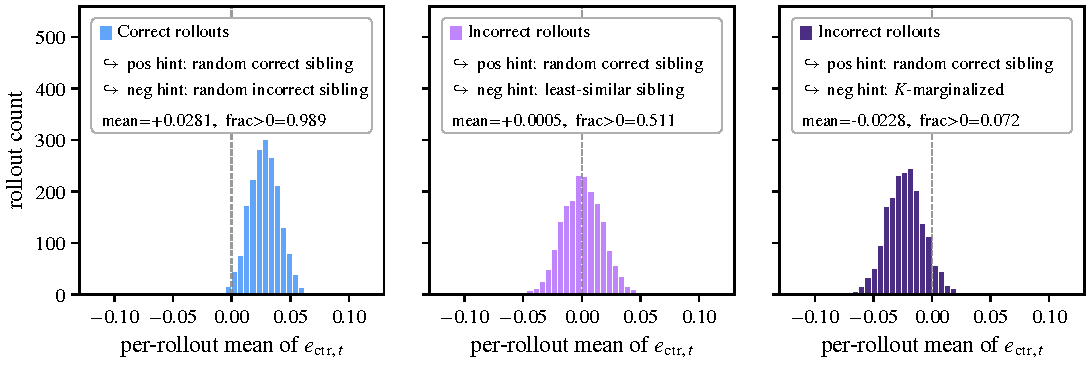
\includegraphics[width=1.0\linewidth]{figs/failure_mode_1.pdf}
    \caption{Rollout-level mean of $e_{\text{ctr},t}$, computed with one positive hint and one or more negative hints. The positive hint is a randomly sampled correct sibling in all three panels; the panels differ in the rollout type and the negative-hint strategy. \textbf{Left:} correct rollouts with a single randomly sampled negative hint, illustrating the expected positive signal of Case~1. \textbf{Middle:} incorrect rollouts with a single LLM-judged least-similar negative hint (the worst case, Case~3). \textbf{Right:} incorrect rollouts with $K$-marginalized negative hints.}
\label{fig:naive-failure-1}
\end{figure}

\paragraph{Empirical validation.}
Figure~\ref{fig:naive-failure-1} confirms the analysis through rollout-level
means of $e_{\text{ctr},t}$. Correct rollouts produce a cleanly positive signal
(left, frac~$>0$~=~0.989), validating Case~1. To isolate Case~3, the middle
panel uses the least-similar negative hint per incorrect $y$ (selected offline
by an LLM judge): the signal is centered at zero, with roughly half the
rollouts bearing the wrong sign. $K$-marginalization (right) restores a cleanly
negative-skewed signal, reducing the wrong-sign rate from $51\%$ to under $8\%$.

\subsection{Self-Referential Collapse and Excluding the Target Rollout}
\label{app:self-hint}

\paragraph{Self-conditioning induces over-confidence.}
Whenever a privileged hint is sampled from student rollouts, the target rollout $y$ itself may be selected as its own hint. Conditioning the teacher on the exact response being evaluated induces extreme over-confidence, making the resulting signal overly sharp and obscuring the token-level distinctions that $e_{\mathrm{ctr},t}$ is intended to capture.

To characterize this effect, we compare conditioning on the target rollout itself with conditioning on another rollout for the same query, considering both correct and incorrect targets. As shown in Figure~\ref{fig:naive-failure-2}, for correct rollouts, a sibling hint leaves the overall distribution largely unchanged, whereas using the target itself as the hint raises the fraction of high-probability tokens ($P_T > 1-10^{-5}$) by roughly $30\%$. For incorrect rollouts, $K$-marginalization mitigates this effect, but including the target among the $K$ candidates still increases the high-probability fraction by about $10\%$.

We therefore exclude the target rollout $y$ from all rollout-derived hint pools. In our setting, this means drawing negative hints from $\mathcal{G}^-\setminus\{y\}$. More generally, if correct student rollouts are used as positive hints, the same exclusion should apply: positive hints should be drawn from $\mathcal{G}^+\setminus\{y\}$.

\begin{figure}[t]
    \centering
    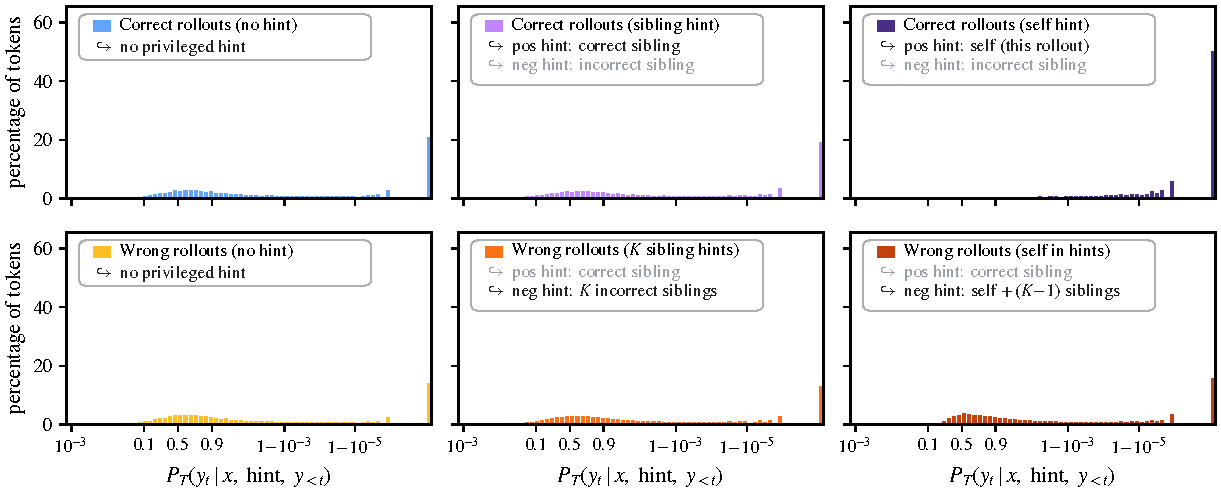
\includegraphics[width=1.0\linewidth]{figs/failure_mode_2.pdf}
    \caption{Distribution of teacher token probabilities $P_T(y_t \mid x, \text{hint}, y_{<t})$ under different hint sources, for correct (top) and incorrect (bottom) rollouts. Using a sibling hint leaves the distribution close to the no-hint case, whereas including the rollout itself as the hint shifts mass toward over-confident, high-probability tokens, motivating its exclusion from the hint pool.}
\label{fig:naive-failure-2}
\end{figure}

\section{Implementation Details}
\label{app:implement-detail}

This section presents the full implementation details that were not fully described in Section~\ref{sec:exp-setup} of the main text.

\subsection{Shared training setup}
\label{app:shared-hparams}

  All methods are implemented on top of the veRL~\citep{sheng2024hybridflow} PPO
  trainer with FSDP2 actor sharding and vLLM rollouts.
  All runs use full-parameter training (no LoRA) on $8\times$H20 GPUs.
  The settings in Table~\ref{tab:shared-hparams} are identical across
  GRPO, OPSD, SDPO, SRPO, RLSD, and RLCSD within a given (task, backbone)
  configuration. Only the per-step loss differs across methods.

  \begin{table}[h]
  \centering
  \small
  \caption{Hyperparameters shared by all six methods. }
  \label{tab:shared-hparams}
  \begin{tabular}{lll}
  \toprule
  Group & Hyperparameter & Value \\
  \midrule
  \multirow{5}{*}{Optimization}
    & Optimizer            & AdamW \\
    & Weight decay         & $0.01$ \\
    & LR warmup (linear)   & $50$ steps \\
    & LR   & $1 \times 10^{-6}$ \\
    & GPUs                 & $8\times$H20 \\
  \midrule
  \multirow{5}{*}{Batching}
    & Per-device batch     & $8$ \\
    & Group size $G$       & $8$ \\
    & PPO mini-batch       & $16$ \\
    & Rollout IS mode      & token-level \\
    & Rollout IS threshold & $2.0$ \\
  \midrule
  \multirow{4}{*}{Rollout sampling}
    & Temperature          & $1.0$ \\
    & Top-$p$ / Top-$k$    & $0.95\ /\ 20$ \\
    & Max prompt length    & $2{,}048$ \\
    & Max completion length & $16{,}384$ \\
  \midrule
  \multirow{5}{*}{Evaluation sampling}
    & Temperature                  & $0.6$ \\
    & Top-$p$ / Top-$k$            & $0.95\ /\ 20$ \\
    & Max completion length        & $38{,}912$ \\
    & Eval batch size              & $16$ \\
    & Samples per query            & $12$ (math, mean@12) / $1$ (K\&K, pass@1) \\
  \bottomrule
  \end{tabular}
  \end{table}



  \subsection{Method-specific hyperparameters}
  \label{app:method-hparams}

  Table~\ref{tab:method-hparams} lists the hyperparameters that vary
  across methods. We follow the \emph{original papers} wherever values are specified there.

\begin{table}[t]
  \centering
  \small
  \caption{Method-specific hyperparameters.}
  \label{tab:method-hparams}
  \resizebox{\textwidth}{!}{%
  \begin{tabular}{llll}
  \toprule
  Method & Hyperparameter & Value & Description \\
  \midrule
  \multirow{2}{*}{GRPO}
    & KL-to-ref coef.        & $10^{-3}$ & coef. on $\mathrm{KL}(\pi_\theta\|\pi_{\text{ref}})$. \\
    & PPO clip $\epsilon$    & $0.2$     & PPO-clip range. \\
  \midrule
  \multirow{7}{*}{OPSD}
    & KL-to-ref coef.        & $0$       & disabled. \\
    & JSD mixing $\beta$     & $0.0$     & $0$ = forward KL, $1$ = reverse KL. \\
    & Vocab clip             & $0.05$    & per-(token, vocab) divergence cap. \\
    & Full-logit distill     & yes       & dense top-$k$ + tail-bucket target. \\
    & Top-$k$                & $100$     & vocab indices per token. \\
    & Tail bucket            & yes       & residual mass outside top-$k$. \\
    & Teacher mode           & fixed     & frozen pretrained checkpoint. \\
  \midrule
  \multirow{7}{*}{SDPO\,/\,SRPO}
    & KL-to-ref coef.        & $0$       & disabled. \\
    & Mixing coef.\ $\alpha$ & $0.5$     & student/teacher mix in JSD target. \\
    & Full-logit distill     & yes       & dense top-$k$ + tail-bucket. \\
    & Top-$k$                & $100$     & vocab indices per token. \\
    & PPO clip ratio         & $2.0$     & IS-ratio clip on distill term. \\
    & EMA decay              & $0.95$    & EMA self-teacher decay. \\
    & Teacher mode           & EMA       & EMA of policy weights. \\
  \midrule
  \multirow{6}{*}{RLSD}
    & KL-to-ref coef.        & $0$       & disabled. \\
    & PPO clip $\epsilon$    & $0.2$     & outer PPO-clip on $\pi_\theta/\pi_{\text{old}}$. \\
    & Evidence clamp $\epsilon_w$ & $0.2$ & clamp on $w_t=\exp(\mathrm{sign}(A)\,(\log\pi_T\!-\!\log\pi_S))$. \\
    & Modulator $\lambda$    & $0.5$     & $\lambda{=}0$: GRPO; $\lambda{=}1$: full modulation. \\
    & $\lambda$ schedule     & $0.5\!\to\!0$ in $50$ steps & linear decay. \\
    & Teacher mode           & snapshot ($\tau_{\text{sync}}{=}10$) & hard copy every $10$ steps. \\
  \midrule
  \multirow{8}{*}{RLCSD (ours)}
    & KL-to-ref coef.        & $0$      & disabled. \\
    & PPO clip $\epsilon$    & $0.2$    & both paths of Eq.~\ref{eq:rlcsd-loss}. \\
    & Slope $\tau$           & $1.3$   & $\tanh$ temperature, Eq.~\ref{eq:rt}. \\
    & Scale $\lambda$        & $0.5$    & overall scale of $r_t$, Eq.~\ref{eq:rt}. \\
    & Mask threshold $\delta$ & $0.02$  & $m_t{=}\mathbb{1}[|r_t|{>}\delta]$, Eq.~\ref{eq:mt}. \\
    & Two-path weight $\eta$  & $0.5$   & modulated-path weight, Eq.~\ref{eq:rlcsd-loss}. \\
    & Neg.\ hints $K$         & $4$     & negative siblings averaged, Eq.~\ref{eq:final-ectr}. \\
    & Teacher mode            & fixed \\
  \bottomrule
  \end{tabular}}
  \end{table}

\section{Vocabulary Partitioning for Task / Style Statistics}
  \label{app:vocab-split}

  This section specifies the token partition of math reasoning tasks used
  in Figures~\ref{fig:ec-task-vs-style} and~\ref{fig:ctr-clean}.

  For each decoded token, we first strip the leading-space marker used by
  the Qwen3 tokenizer and lowercase the result. The token is then sent
  through the following rules in order, returning at the first match:

  \begin{enumerate}
  \itemsep0em
  \item[(1)] empty or whitespace-only $\rightarrow$ \textbf{style};
  \item[(2)] matches any of the math regexes
             (a digit \texttt{\textbackslash d};
              an arithmetic operator in
              \texttt{+\,-\,=\,*\,/\,<\,>\,×\,÷\,$\leq$\,$\geq$\,$\neq$};
              a LaTeX command \texttt{\textbackslash[A-Za-z]+};
              a double backslash;
              or one of \texttt{\$\,\textasciicircum\,\_})
             $\rightarrow$ \textbf{task};
  \item[(3)] the normalized form is in the math wordlist
             \texttt{\{mod, prime, factor, gcd, lcm, log, ln, sin, cos,
             tan, exp, integral, sqrt, boxed, frac, sum, prod, pi, alpha,
             beta, gamma, theta, delta, lambda, mu, sigma, infty, leq,
             geq, neq, cdot, times, div\}}
             $\rightarrow$ \textbf{task};
  \item[(4)] pure punctuation or a literal newline token
             ({\tt \textbackslash n}, {\tt \textbackslash\textbackslash n})
             $\rightarrow$ \textbf{style};
  \item[(5)] the normalized form is in the discourse wordlist
             (connectives \texttt{therefore, so, thus, hence, then, because,
             since}; hedges \texttt{wait, maybe, perhaps, seems, okay, ok,
             well, now, first, next, finally, actually, alternatively,
             however}; scaffolding \texttt{step, answer, let, lets};
             closed-class function words \texttt{is, are, us, we, the, a,
             an, of, to, for, in, on, by, at, as, and, or, but, if, yes,
             no, this, that, these, those, it, its, be, been, being, have,
             has, had, do, does, did, will, would, should,
             could, can, may})
             $\rightarrow$ \textbf{style};
  \item[(6)] otherwise $\rightarrow$ \textbf{neutral}.
  \end{enumerate}


\section{Computational Cost Analysis}

RLCSD introduces additional teacher-side computation compared with one-sided self-distillation methods, since it evaluates the teacher on both a correct hint and multiple wrong hints to form the contrastive signal. This extra cost is reflected in the \texttt{teacher log prob} time in Table~\ref{tab:wall_clock}: RLCSD spends \(14.210\)s per step on teacher scoring, compared with about \(9\)s for one-sided methods such as RLSD and OPSD.

However, this overhead is small compared with the dominant cost of autoregressive rollout generation. RLCSD spends \(473.89\)s per step on \texttt{gen}, so the extra teacher scoring is only a minor fraction of the generation cost. In other words, although RLCSD requires more teacher forwards, these forward-only evaluations add relatively little wall-clock overhead compared with sampling long reasoning trajectories.

More importantly, the end-to-end step time remains favorable. As shown in Table~\ref{tab:wall_clock}, RLCSD is the \emph{third fastest} method overall, behind only GRPO and RLSD. In particular, it is faster than dense-distillation baselines such as OPSD, SDPO, and SRPO. A likely reason is that these methods perform dense token-level distillation over the vocabulary during training, which makes the optimization stage itself much more expensive than the sampled-token modulation used in RLCSD and RLSD. 

\begin{table}[h]
\centering
\small
\caption{Average wall-clock time per training step (seconds) on math reasoning task, using Qwen3-4B as the base model. RLCSD spends more time on \texttt{teacher\_log\_prob} because it uses additional wrong-hint teacher forwards, but this overhead is small relative to rollout generation (\texttt{gen}). In total step time, RLCSD remains the third fastest method overall.}
\label{tab:wall_clock}
\begin{tabular}{lccc}
\toprule
Method & Gen (s/step) & Teacher log prob (s/step) & Total step (s/step) \\
\midrule
GRPO  & 503.78 & --     & 759.01  \\
OPSD  & 413.92 & 9.552  & 1035.54 \\
SDPO  & 495.64 & 9.701  & 961.14  \\
SRPO  & 411.01 & 9.566  & 1011.51 \\
RLSD  & 412.27 & 9.485  & 812.84  \\
RLCSD & 473.89 & 14.210 & 891.55  \\
\bottomrule
\end{tabular}
\end{table}

\section{Additional Results on Agentic Tasks}
\label{app:agentic}

\paragraph{Settings.} We evaluate Qwen3-4B on ALFWorld~\citep{shridhar2020alfworld} and WebShop~\citep{yao2022webshop}. We allow at most 30 interaction steps per episode on ALFWorld and 20 on WebShop, where each step consists of an agent action and the corresponding environment response. For both benchmarks, we enable thinking mode and impose a trajectory budget of 16,384 tokens, counting both model outputs and subsequent environment observations. At evaluation time, we sample one trajectory per task with a temperature of 0.6; we use top-$p$ of 1.0 without top-$k$ filtering for ALFWorld, and top-$p$ of 0.95 with top-$k$ of 20 for WebShop. For ALFWorld, we report overall success rate and success rates on the seen and unseen splits. For WebShop, we report the average reward, which includes partial credit and ranges from 0 to 1, and the success rate, defined as the fraction of episodes receiving a reward of 1. All success rates are reported as percentages.

\begin{table}[t]
\centering
\caption{Results on agentic tasks using Qwen3-4B. ALFWorld metrics are success rates (\%). WebShop Score is the average reward on a scale of $[0,1]$, and Success is the percentage of episodes receiving a reward of 1. Higher is better for all metrics. \textbf{Bold} marks the best result in each column, and \underline{underline} marks the second-best result.}
\label{tab:agentic}
\small
\setlength{\tabcolsep}{8pt}
\begin{tabular}{lccccc}
\toprule
& \multicolumn{3}{c}{\textbf{ALFWorld}}
& \multicolumn{2}{c}{\textbf{WebShop}} \\
\cmidrule(lr){2-4}\cmidrule(lr){5-6}
\textbf{Method}
& Overall (\%) & Seen (\%) & Unseen (\%)
& Score & Success (\%) \\
\midrule
Base  & 43.06 & 45.00 & 41.04 & 0.5081 & 18.4 \\
GRPO  & \underline{47.44} & 48.57 & 46.26 & 0.5170 & 18.8 \\
OPSD  & 46.35 & 42.85 & \textbf{50.00} & 0.5164 & 18.5 \\
SDPO  & 46.35 & \textbf{50.71} & 41.79 & \underline{0.5225} & 18.6 \\
SRPO  & 45.98 & 46.42 & 45.52 & 0.5194 & 18.7 \\
RLSD  & 45.62 & 43.57 & \underline{47.76} & 0.5218 & \underline{19.1} \\
\rowcolor{gray!30}
\textbf{RLCSD} & \textbf{48.17} & \underline{49.28} & 47.01 & \textbf{0.5300} & \textbf{19.4} \\
\bottomrule
\end{tabular}
\end{table}

\paragraph{Results.} As shown in Table~\ref{tab:agentic}, RLCSD achieves the highest overall success rate on ALFWorld and the best average reward and success rate on WebShop. On ALFWorld, RLCSD reaches 48.17\% overall success, outperforming the base model by 5.11 percentage points and the strongest baseline, GRPO, by 0.73 percentage points. Although SDPO and OPSD achieve the highest success rates on the seen and unseen splits, respectively, RLCSD performs consistently across both splits, yielding the best overall result. On WebShop, RLCSD achieves an average reward of 0.5300 and a success rate of 19.4\%, exceeding the strongest baselines for these metrics by 0.0075 and 0.3 percentage points, respectively. These results show consistent, albeit modest, improvements over the competing methods across both environments.


\section{Sensitivity Analysis of Hyperparameters in RLCSD}
\label{app:hyperparameter}

We investigate how RLCSD's hyperparameters affect token selection and training behavior using Qwen3-8B on DeepMath. The five hyperparameters are the number of negative hints $K$, the soft-normalization temperature $\tau$, the modulation scale $\lambda$, the selection threshold $\delta$, and the modulated-path weight $\eta$. Our default configuration is
\begin{equation}
(K,\tau,\lambda,\delta,\eta)=(4,1.3,0.5,0.02,0.5).
\end{equation}
We first analyze their direct effects on fixed contrastive signals, then examine the default training dynamics and controlled comparisons in which one hyperparameter is varied at a time.

\subsection{How the Hyperparameters Affect the Learning Signal}

\paragraph{Token selection depends on a joint effective threshold.}
RLCSD transforms the raw contrastive signal into a bounded modulation and selects tokens according to
\begin{equation}
r_t=\lambda\tanh\left(\frac{e_{\mathrm{ctr},t}}{\tau}\right),
\qquad
m_t=\mathbf{1}(|r_t|>\delta).
\end{equation}
For $\tau>0$ and $0<\delta<\lambda$, the selection criterion is equivalent to
\begin{equation}
m_t=\mathbf{1}\left(|e_{\mathrm{ctr},t}|>h_{\mathrm{eff}}\right),
\qquad
h_{\mathrm{eff}}
=\tau\operatorname{arctanh}\left(\frac{\delta}{\lambda}\right).
\end{equation}
Thus, $\tau$, $\lambda$, and $\delta$ jointly determine selection coverage. On fixed raw signals, increasing $\tau$ or $\delta$ raises the effective threshold and selects fewer tokens, whereas increasing $\lambda$ lowers it and selects more tokens. The default configuration corresponds to $h_{\mathrm{eff}}\approx0.0520$.

Table~\ref{tab:hyperparameter-mechanism} summarizes these analytical relationships. Different configurations can produce identical selection masks while assigning different modulation magnitudes. For example, doubling $\lambda$ and halving $\delta$, considered separately from the same default configuration, produce the same effective threshold at fixed $\tau$. However, only the former scales the modulation values.

\begin{table}[t]
\centering
\caption{Analytical effects of changing one hyperparameter from the default configuration. The effective threshold $h_{\mathrm{eff}}$ and local gain $\lambda/\tau$ are calculated from the modulation formula. Selection trends assume fixed raw contrastive signals and describe non-strict changes relative to the default configuration.}
\label{tab:hyperparameter-mechanism}
\small
\setlength{\tabcolsep}{7pt}
\begin{tabular}{lcccc}
\toprule
Configuration
& $h_{\mathrm{eff}}$
& Local gain $\lambda/\tau$
& Bound $\lambda$
& Selection coverage \\
\midrule
Default          & 0.0520 & 0.3846 & 0.50 & --- \\
\midrule
$\tau=0.65$      & 0.0260 & 0.7692 & 0.50 & Increases \\
$\tau=2.6$       & 0.1041 & 0.1923 & 0.50 & Decreases \\
\midrule
$\lambda=0.25$   & 0.1042 & 0.1923 & 0.25 & Decreases \\
$\lambda=1.0$    & 0.0260 & 0.7692 & 1.00 & Increases \\
\midrule
$\delta=0.01$    & 0.0260 & 0.3846 & 0.50 & Increases \\
$\delta=0.04$    & 0.1042 & 0.3846 & 0.50 & Decreases \\
\midrule
$\eta=0.25$      & 0.0520 & 0.3846 & 0.50 & Unchanged \\
$\eta=1.0$       & 0.0520 & 0.3846 & 0.50 & Unchanged \\
\bottomrule
\end{tabular}
\end{table}

\paragraph{Modulation strength differs from selection coverage.}
For small $|e_{\mathrm{ctr},t}|/\tau$, the modulation is approximately linear:
\begin{equation}
r_t\approx\frac{\lambda}{\tau}e_{\mathrm{ctr},t}.
\end{equation}
The ratio $\lambda/\tau$ controls the local gain, while $\lambda$ bounds the modulation magnitude. Increasing $\lambda$ scales every modulation value proportionally. Decreasing $\tau$ also strengthens the modulation, but pushes more tokens toward saturation and compresses differences among large raw signals.

In contrast, changing $\delta$ leaves every $r_t$ unchanged and affects only selection. A larger $\delta$ therefore retains fewer, stronger signals without changing the average modulation magnitude over all tokens. For $\lambda$ and $\tau$, changes in modulation magnitude and selected-set membership occur together, so the average magnitude among selected tokens need not follow the same trend as the all-token average. The sign-preserving clamp further limits the effective advantage change when a modulation would otherwise reverse the outcome-based update direction.

\paragraph{Negative-hint marginalization controls estimation variability.}
The parameter $K$ acts upstream by changing the negative-branch estimate:
\begin{equation}
e_{\mathrm{ctr},t}
=
\log p_{c,t}
-
\log\left(\frac{1}{K}\sum_{k=1}^{K}p_{w,k,t}\right),
\end{equation}
where $p_{c,t}$ and $p_{w,k,t}$ denote teacher probabilities under the correct and incorrect references, respectively. Under independent sampling, the variance of the negative-branch probability mean decreases as $1/K$. Increasing $K$ can therefore reduce sensitivity to individual negative hints and improve coverage of the error modes represented in the hint pool. However, it does not imply a monotonic change in the absolute contrastive signal or the selected-token ratio, because both depend on the sampled probabilities and the subsequent logarithm.

\paragraph{Path weighting interacts with selection sparsity.}
For a rollout with nonempty unmodulated and modulated token sets, the objective is
\begin{equation}
J
=
\frac{1}{|\mathcal U|}
\sum_{t\in\mathcal U}\psi_t(A_{\mathrm{ORM}})
+
\frac{\eta}{|\mathcal M|}
\sum_{t\in\mathcal M}\psi_t(\widetilde A_t).
\end{equation}
Writing $q=|\mathcal M|/(|\mathcal U|+|\mathcal M|)$, the ratio of per-token normalization weights is
\begin{equation}
\frac{\eta/|\mathcal M|}{1/|\mathcal U|}
=
\eta\frac{1-q}{q}.
\end{equation}
Selecting fewer tokens therefore concentrates the modulated-path weight on a smaller subset rather than proportionally reducing its nominal weight. At $\eta=0.5$, this ratio is $2.0$ for $q=0.2$ and approximately $1.17$ for $q=0.3$, before accounting for advantage magnitudes and PPO clipping.

Unlike $\lambda$, $\eta$ does not directly change the signal or the selection mask. It scales the entire modulated path, including the outcome-level anchor within $\widetilde A_t$. During training, however, changing $\eta$ can indirectly alter subsequent selection statistics by changing the policy and its rollout distribution.

\subsection{Training Dynamics under the Default Configuration}

Table~\ref{tab:default-dynamics} reports the default configuration's training statistics across three windows. The selected-token ratio remains close to $28\%$--$30\%$, decreasing from $30.01\%$ over steps 1--50 to $28.24\%$ over steps 351--400. Response length is maintained, changing from approximately $9{,}423$ to $9{,}617$ tokens, while training reward remains comparable across the middle and late stages. Actor entropy decreases from $0.321$ to $0.183$ without an accompanying collapse in response length. These observations characterize the default configuration as maintaining selective modulation throughout training while preserving extended responses.

\begin{table}[t]
\centering
\caption{Training dynamics of Qwen3-8B on DeepMath under the default RLCSD configuration. Each entry is the mean of the logged per-step metric over the indicated training window.}
\label{tab:default-dynamics}
\small
\setlength{\tabcolsep}{10pt}
\begin{tabular}{lccc}
\toprule
Metric & Steps 1--50 & Steps 201--250 & Steps 351--400 \\
\midrule
Selected tokens (\%) & 30.01 & 28.62 & 28.24 \\
Response length     & 9423  & 9346  & 9617  \\
Training reward     & 0.736 & 0.753 & 0.749 \\
Actor entropy       & 0.321 & 0.201 & 0.183 \\
\bottomrule
\end{tabular}
\end{table}

\subsection{Controlled Hyperparameter Comparisons}

\paragraph{Evaluation protocol.}
We vary one hyperparameter at a time while keeping the remaining settings and training budget fixed. We report the selected-token ratio, response length, training reward, and actor entropy averaged over steps 351--400, together with AIME25 mean@12 at step 400. These training-level measurements capture both the direct effects described above and the indirect effects of changes in the learned policy.

\begin{table}[t]
\centering
\caption{Hyperparameter sensitivity of RLCSD on Qwen3-8B and DeepMath. Each configuration changes one parameter from the default setting. Training statistics are averaged over steps 351--400; AIME25 mean@12 is evaluated at step 400.}
\label{tab:hyperparameter-training}
\small
\resizebox{0.8\textwidth}{!}{%
\begin{tabular}{lccccc}
\toprule
Configuration
& Selected (\%)
& Length (tokens)
& Reward
& Entropy
& AIME25 (\%) \\
\midrule
Default             & 28.24 & 9617  & 0.749 & 0.183 & 69.72 \\
\midrule
$K=1$               & 32.67 & 9148  & 0.731 & 0.207 & 66.94 \\
$K=2$               & 29.83 & 9486  & 0.743 & 0.192 & 68.89 \\
\midrule
$\tau=0.65$         & 39.56 & 10083 & 0.744 & 0.216 & 68.61 \\
$\tau=2.6$          & 18.72 & 9324  & 0.738 & 0.174 & 68.06 \\
\midrule
$\lambda=0.25$      & 19.15 & 9408  & 0.741 & 0.178 & 68.33 \\
$\lambda=1.0$       & 40.38 & 10426 & 0.736 & 0.231 & 67.78 \\
\midrule
$\delta=0.01$       & 38.91 & 9702  & 0.747 & 0.189 & 69.17 \\
$\delta=0.04$       & 18.46 & 9538  & 0.750 & 0.181 & 70.00 \\
\midrule
$\eta=0.25$         & 27.63 & 9361  & 0.740 & 0.176 & 68.61 \\
$\eta=1.0$          & 29.47 & 10054 & 0.745 & 0.204 & 69.44 \\
\bottomrule
\end{tabular}%
}
\end{table}

\paragraph{Selection coverage follows the effective-threshold analysis.}
The changes in selected-token ratio agree with the predicted directions. Decreasing $\tau$ to $0.65$, increasing $\lambda$ to $1.0$, or decreasing $\delta$ to $0.01$ expands coverage to approximately $39\%$--$40\%$. The opposite changes reduce coverage to approximately $18\%$--$19\%$. Although these relationships are derived for fixed raw signals, their directions remain evident after training. Across these configurations, AIME25 ranges from $67.78\%$ to $70.00\%$, indicating that substantial changes in selection coverage do not translate into proportional changes in validation performance.

\paragraph{Multiple negative hints improve performance.}
Increasing $K$ from 1 to 2 and 4 improves AIME25 from $66.94\%$ to $68.89\%$ and $69.72\%$, respectively. Training reward also increases from $0.731$ to $0.743$ and $0.749$. These results are consistent with the benefit of a more reliable negative-branch estimate. The incremental accuracy gain decreases from $1.95$ points for $K=1$ to $K=2$ to $0.83$ points for $K=2$ to $K=4$, supporting the use of multiple hints while suggesting diminishing gains within the tested range.

\paragraph{Stronger modulation does not necessarily improve accuracy.}
Increasing $\lambda$ to $1.0$ or decreasing $\tau$ to $0.65$ produces longer responses than the default configuration, reaching $10{,}426$ and $10{,}083$ tokens on average, respectively. However, their AIME25 scores decrease to $67.78\%$ and $68.61\%$. Weaker modulation also yields lower scores: $\lambda=0.25$ and $\tau=2.6$ achieve $68.33\%$ and $68.06\%$. These comparisons support balancing modulation strength rather than maximizing it, and show that longer responses alone do not guarantee better reasoning performance.

\paragraph{Sparser selection can preserve performance.}
Increasing $\delta$ to $0.04$ reduces the selected-token ratio from $28.24\%$ to $18.46\%$ while maintaining comparable AIME25 performance ($70.00\%$ versus $69.72\%$). Decreasing $\delta$ to $0.01$ expands coverage to $38.91\%$ but yields $69.17\%$. These results suggest that broader coverage is not always necessary: independent normalization allows a smaller selected set to retain substantial influence on optimization. The small accuracy difference between $\delta=0.04$ and the default does not establish a clear preference between them.

\paragraph{Modulated-path weighting has a moderate effect in the tested range.}
Changing $\eta$ to $0.25$ or $1.0$ yields AIME25 scores of $68.61\%$ and $69.44\%$, respectively, compared with $69.72\%$ for the default. The selected-token ratio remains relatively close to the default, ranging from $27.63\%$ to $29.47\%$, consistent with $\eta$ affecting selection only indirectly through training. These comparisons support $\eta=0.5$ as a reasonable operating point, while the performance differences do not indicate that it is uniquely optimal.